\chapter{Reinforcement learning and Self play approach}
\section{Introduction}
\section{Reinforcement Learning}
\subsection{Definition}
\citeauthor{RLIntroduction} \cite[Chapter.~1]{RLIntroduction} gave an excellent in-depth definition, which not only defines what \acrfull{rl} is, but also compare it with other \acrfull{ml} methods.
\newline We will summarize it as follow:
\begin{definition}
	RL deals with opti
\end{definition}
\begin{figure}
	\centering
	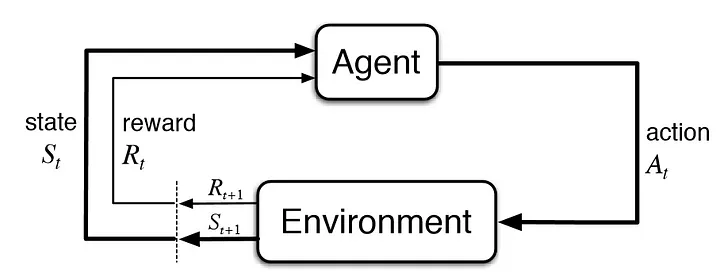
\includegraphics[width= 0.8\textwidth]{Figures/RLDiagram.png}
	\caption{A Reinforcement Learning system}
\end{figure}
\subsection{Theory}
\subsubsection{Single Agent}
In most settings, the theory of reinforcement learning deals with environments where we would like to optimize a single agent. This is called single-agent reinforcement learning. This is usually modeled with a Markov Decision Process \cite[Chapter~3]{RLIntroduction}.
\newline Reinforcement Learning methods differ by their underlying assumptions

\subsubsection{Multi Agent}
In our case, a Mean Payoff Game can be modelled in the reinforcement learning setting as a Stochastic Game\footnote{Also known as Markov Game} \cite{StochasticGames}.
\newline This is a powerfull tool, as it can also model the stochastic version of mean payoff games \cite{StochasticMPG}. 

\subsubsection{Markov Chains}
\subsubsection{Markov Reward Process}
\subsection{\acrshort{rl} formalization of a \acrshort{mpg}}
\subsubsection{State abstraction}
Remember that an \acrshort{mpg} is modeled as a tuple $G=(V,E,W,s,p).$
\newline For the reinforcement learning setting, we will define 


\section{Monte Carlo Tree Search}
\acrfull{mcts} is an advanced algorithm in decision making that appeared in \citedate{MCTSOriginal}. \citeauthor{MCTSOriginal} first coined the term \acrshort{mcts} as application of Monte-Carlo methods to game-tree search \cite{MCTSOriginal}. It is an important algorithm for adversial search. that had a huge success at improving the competence of Go engines to a master level \cite{GoMaster}. This alone was a feat considering that previous state of the are alpha-beta implementations were unable to get past beginner level. 

Much development occured to \acrshort{mcts}, which made it a little hard to define. \citeauthor{RLIntroduction} gave the following definition \cite[section.~8.8]{RLIntroduction}: \textit{``\acrfull{mcts} is a planning algorithm that accumulates value estimates obtained from Monte Carlo simulations in order to successively direct simulations towards more highly-rewarded trajectories."}

This definition alone is unsatisfactory, \citeauthor{AIModernApproach} gave an intuitive explanation \cite[Section~6.4]{AIModernApproach} of how \acrfull{mcts} works for a game. And we will base this section on his work. 
 
Essentially, \acrshort{mcts} consists of the following $4$ steps:
\subsection{Selection}
Starting at the root, we choose a child following a \textbf{selection policy} $\Pi^{\text{selection}}$, and repeat the step until arriving to a leaf node.
\begin{algorithm}
	\caption{Selection algorithm for \acrshort{mcts}}\label{alg:MCTSSelection}
	\begin{algorithmic}
		\Require $r$ the root of the \acrshort{mcts}.
		\Require $\Pi^{\text{selection}}$ the current selection policy..
		\Ensure $s$ a leaf of the \acrshort{mcts}.
		\State $s\leftarrow r$
		\While{$\Not \ \text{leaf}(r)$}
			\State  $s\leftarrow \Pi^{\text{selection}}(r)$
		\EndWhile
		\State \Return $s$
	\end{algorithmic}
\end{algorithm}

\subsection{Expansion}
At the selected leaf $s$, we grow the \acrshort{mcts} by adding a new child $t$ that is a result of some action $a$ from $s.$

\begin{algorithm}
	\caption{Expansion algorithm for \acrshort{mcts}}\label{alg:MCTSExpansion}
	\begin{algorithmic}
		\Require $s$ a leaf \acrshort{mcts}.
		\Require $H$ the mean reward of each node in the \acrshort{mcts}
		\Require $T$ the number of simulations for each node in the \acrshort{mcts} 
		\Ensure $t$ a new child of $s$
		\State  $C\leftarrow \text{expand\_children}(s)$ \Comment{Generate a set of children from $s$}
		\For {$c \in C$}
			\State $T(c)\leftarrow 0$ \Comment{$c$ is currently visited $0$ times}
			\State $H(c)\leftarrow \boldsymbol{0}$ \Comment{The reward of each player at $c$ is initialized to $0$}
		\EndFor
		\State \text{$t\leftarrow \text{choose}(C)$} \Comment{Choose a child from $C$}
		\State \Return $t$
	\end{algorithmic}
\end{algorithm}

\subsection{Simulation}
Starting from the new child $t,$ we perform a complete playout, that is, we choose moves for all players according to the playout policy $\Pi^{\text{playout}}.$
\newline The generated sequence of nodes in the playout will not be recorded in the \acrshort{mcts}
\begin{algorithm}
	\caption{Simulation algorithm for \acrshort{mcts}}\label{alg:MCTSSimulation}
	\begin{algorithmic}
		\Require $t$ the new child of the \acrshort{mcts}.
		\Require $\Pi^{\text{playout}}$ the current playout policy..
		\Ensure $W$ the cumulative rewards after the playout for each player.
		\State  $s\leftarrow \text{state}(t)$ \Comment{get the current state}
		\State  $p\leftarrow \text{state}(t)$ \Comment{get the current player}
		\State $W\leftarrow \boldsymbol{0}$ 
		\While{$\Not \ \text{terminal}(s)$}
		\State  $a\leftarrow \Pi^{\text{playout}}(s,p)$
		\State $(s,p,U) \leftarrow \text{apply}(s,a)$ \Comment{Apply action $a$ at state $s$, and getting reward $U$}
		\State $W\leftarrow W+U$
		\EndWhile
		\State \Return $W$
	\end{algorithmic}
\end{algorithm}


\subsection{Backpropagation}
Once a simulation is complete, we use its result to update the all search nodes going from $t$ up to the root.
\begin{algorithm}[h]
	\caption{Backpropagation algorithm for \acrshort{mcts}}\label{alg:MCTSBackpropagation}
	\begin{algorithmic}
		\Require $t$ the new child of the \acrshort{mcts}.
		\Require $W$ the reward after the simulation.
		\Require $W'$ the cumulative reward up to node $t$
		\Require $H$ the mean reward of each node in the \acrshort{mcts}
		\Require $T$ the number of simulations for each node in the \acrshort{mcts}
		\While{$\Not \ \text{root}(s)$}
		\State $T(s)\leftarrow T(s)+1$ \Comment{Increment the number of visits of $s$}
		\State $H(s)\leftarrow H(s) - \frac{W+W'-H(s)}{T(s)}$  \Comment{Update the mean reward at $s$}
		\State $s\leftarrow \text{parent}(s)$ \Comment{Go to the parent node}
		\EndWhile
		\State \Return $W$
	\end{algorithmic}
\end{algorithm}
\FloatBarrier
\subsection{Wrapping up}
Once we have the $4$ elements of \acrshort{mcts}, the full algorithm will be just repeating these steps in order until certain desired condition is satisfied. In practice, most implementations use the following conditions for halting the  algorithm:
\begin{itemize}
	\item Execution time exceeds some threshold $T$
	\item Total number of simulations (at root) exceeds some threshold $N$
\end{itemize}

\begin{algorithm}
	\caption{\acrshort{mcts} Algorithm}\label{alg:MCTS}
	\begin{algorithmic}
		\Require $\text{state}$ some state of the game
		\Ensure An action $a\in \text{actions}(\text{state})$
		\State $r\leftarrow \text{tree}(\text{state})$
		\While {Exit condition not satisfied}
		\State $s\leftarrow \text{select}(r)$
		\State $t\leftarrow \text{expand}(s)$
		\State $W\leftarrow \text{simulate}(t)$
		\State $\text{backpropagation}(t,W)$
		\EndWhile
		\State \Return $a\leftarrow \displaystyle \argmax_{a\in \text{actions}(\text{state})}T(a)$ \Comment{Get the most visited action}
	\end{algorithmic}
\end{algorithm}
\begin{figure}
	\centering
	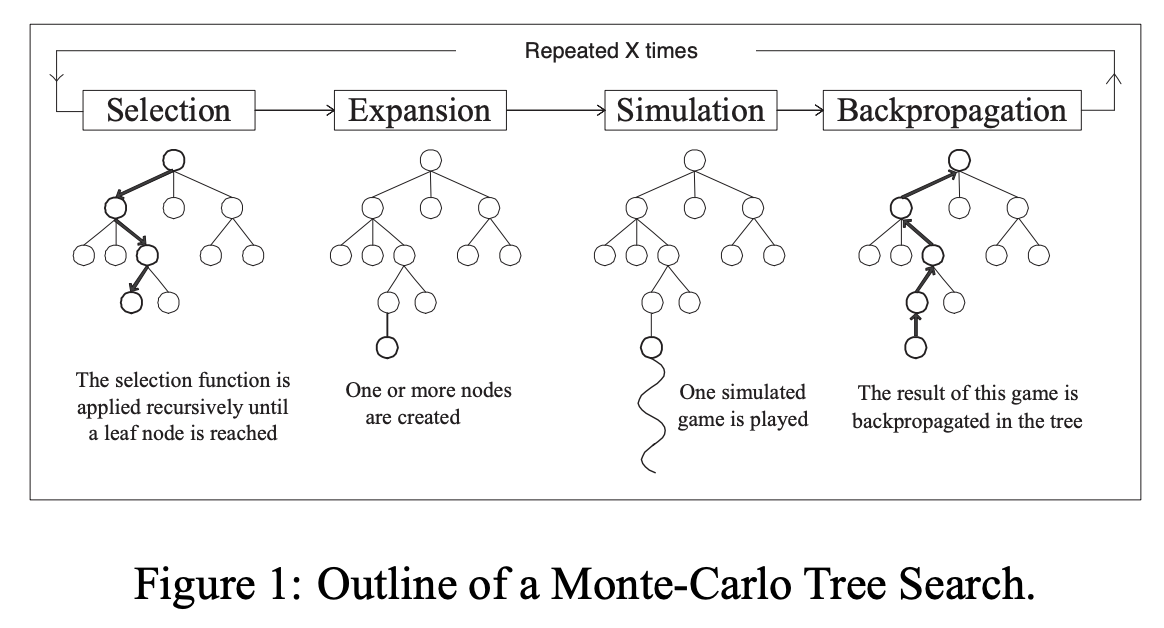
\includegraphics[width=0.75\textwidth]{Figures/MCTS.png}
	\caption{One iteration of a \acrshort{mcts} algorithm}
\end{figure}

\section{Model based \acrshort{mcts}}
\label{section:RL:ModelBasedMCTS}
While we explained how \acrshort{mcts} works in the previous section, some components were left without much discussion:
\begin{enumerate}
	\item The selection policy $\Pi^{\text{selection}}$
	\item The playout policy $\Pi^{\text{playout}}$
	\item Children creation
\end{enumerate}
This was deliberate, as the full power of $\acrshort{mcts}$ requires a good choice of the components, especially $\Pi^{\text{selection}}$ and $\Pi^{\text{playout}}.$

In our case, both functions will be based on the model $\mathcal{M}$ that we designed in chapter \ref{section:ModelDesign} and illustrated in figure \ref{fig:ModelArchitecture}.

Remember that our model $\mathcal{M}$ takes a \acrshort{mpg}\footnote{In fact, it takes a batch of \acrshortpl{mpg}, but this can be easily migitated.}, and produces two outputs:
\begin{enumerate}
	\item The predicted evaluation $v.$
	\item The predicted strategy $\Pi.$
\end{enumerate}
Both of these terms will be used in the \acrshort{mcts}.

\subsection{Create children}
In this version of \acrshort{mcts}, create children will return the list of all adjacent states. It does also apply an optional Dirichlet noise $\mathcal{D}(\alpha)$ if the current node is root.

\begin{algorithm}[H]
	\caption{Create children}\label{alg:CreateChildren}
	\begin{algorithmic}
		\Require $h$ current
		 node
		 \Require Dirichlet noise parameter $\alpha\in\mathbb{R}_+$
		 \Require Exploration noise parameter $\varepsilon\in[0,1]$
		 \Require Prior distribution $\Pi$
		\Ensure A list of children $C$
		\Ensure Optionally update $\Pi$
		\State $G=(V,E,W,s,p)$ is the underlying \acrshort{mpg} related to node $h$
		\State $m\leftarrow \lvert \Adj s \rvert$
		\If {$\text{root}(h)$}
			\State generate $\nu\sim \mathcal{D}(\alpha \ones_m)$ \Comment{$\ones_m \in \mathbb{R}^m$ is the vector of ones}
			\For {$(v,x)\in \zip(\Adj s,\nu)$}
				\State $\Pi(v)\leftarrow (1-\varepsilon)\Pi(v) + \varepsilon x$
			\EndFor
		\EndIf
		\State $C\leftarrow \varnothing$
		\For {$t\in \Adj s$}
			\State $G'\leftarrow (V,E,W,t,\bar{p})$
			\State $\text{append}(C,G')$
		\EndFor
		\State \Return $C$
	\end{algorithmic}
\end{algorithm}

\subsection{Playout Policy}
\label{section:RL:ModelBased:PlayoutPolicy}
In Alpha Zero's implementation of \acrshort{mcts} \cite{AlphaGo}, the playout policy is exactly the predicted distribution $\Pi.$

Also, the simulation algorithm \ref{alg:MCTSSimulation} was modified to only play one move:

\begin{algorithm}[H]
	\caption{Alpha Zero \acrshort{mcts} Simulation}\label{alg:AZSimulation}
	\begin{algorithmic}
		\Require $t$ the new child of the \acrshort{mcts}.
		\Require $\mathcal{M}$ the neural network model
		\Ensure $W$ the cumulative rewards after the playout for each player.
		\State  $G\leftarrow \text{MPG}(t)$ \Comment{get the current state}
		\State  $p\leftarrow \text{player}(t)$ \Comment{get the current player}
		\If {$p$ is $\Min$}
			\State $G\leftarrow \bar{G}$
		\EndIf
		\State $(v,\Pi)\leftarrow \mathcal{M}(G)$
		\If {$p$ is $\Min$}
			\State $v\leftarrow -v$
		\EndIf
		\State $W\leftarrow v$
		\Return $W$
	\end{algorithmic}
\end{algorithm}
\FloatBarrier
\subsection{Selection Policy}
\label{section:RL:ModelBased:SelectionPolicy}
\begin{algorithm}[H]
	\caption{model-based \acrshort{mcts} playout policy}\label{alg:SelectionPolicy}
	\begin{algorithmic}
		\Require $h$ current node 
		\Require $C\in\mathbb{R}_+$ exploration parameter
		\Ensure An child \acrshort{mpg} $G'$
		\State $Z\leftarrow \boldsymbol{0}$
		\For {$c\in \text{children}(h)$}
			\State $Z(c)\leftarrow \PUCT(c,h,\Pi(c),C)$
		\EndFor
		\State \Return $\displaystyle c \leftarrow \argmax_{c\in \text{children}(h)}Z(c)$
	\end{algorithmic}
\end{algorithm}
Here $\PUCT$ is defined as follow:
\begin{equation}
	\label{eqn:PUCT}
	\PUCT(c,h,\Pi(c),C) = H(c) + C\cdot \Pi(c) \cdot \frac{\sqrt{N(h)}}{N(c)+1}
\end{equation}
Here $H(c)$ is the reward of the current player at node $c$.

The equation \eqref{eqn:PUCT} was defined in the Alpha Go paper \cite{AlphaGo} as a model-based variant of $\UCT$ \cite{UCT}. We show the latter's expression to show the differnece between vanilla \acrshort{mcts} and model-based \acrshort{mcts}:
\begin{equation*}
	\UCT(c,h,C) =  H(c) + C\cdot \frac{\log {N(h)}}{N(c)+1}
\end{equation*}

In fact, the additional term $\Pi(c)$ is used to weight the children selection by the prior distribution $\Pi,$ and we believe that using the square root instead of the logarithmic function was deliberate to boost exploration.

\subsection{Wrapping up}
Our model-based \acrshort{mcts} is heavily inspired from the one used at Alpha Zero.

It uses the algorithm \ref{alg:MCTS} with a threshold number of iterations $N$ as exit condition\footnote{This applies to the model training phase. While deploying the algorithm, we can use a different exit condition.}. It avoids complete rollouts, and instead uses the simulation algorithm \ref{alg:AZSimulation} that uses the model $\mathcal{M}$.

Also, the predictions of model $\mathcal{M}$ are directly used in the selection policy defined at section \ref{section:RL:ModelBased:SelectionPolicy} and the playout policy defined at section \ref{section:RL:ModelBased:PlayoutPolicy}.
\subsection{Updating model}
Once the \acrshort{mcts} algorithm terminates. We get for each node a new estimates of both the strategy and the evaluation.
\subsubsection{Evaluation estimate}
The term $H$ used in the \acrshort{mcts} is used for the expected reward for the algorithm. Now as each node $t$ of the tree encodes a \acrshort{mpg} $G,$ $H(t)$ will be the updated estimate of the evaluation:
\begin{equation*}
	v(G)=\mathcal{M}(G)_{\text{evaluation}}
\end{equation*}

For that, we will denote the updated value as $v'(G)=H(t)$

\subsubsection{Strategy estimate}
To illustrate our point, we will need the following definitions:
\begin{itemize}
	\item Let $t$ be a node.
	\item Let $G=(V,E,W,s,p)$ be the \acrshort{mpg} encoded by $t.$
	\item Let $a\in \Adj s$ be an action eligible from $t.$
	\item Let $c$ be the\footnote{It is unique as an \acrshort{mpg} is deterministic. For a stochastic \acrshort{mpg}, which is out of the scope of this report, one should do a more careful analysis.} node resulting from applying $a$
\end{itemize}

Now, we want an esimtate of the strategy implied by the \acrshort{mcts}. In fact, the  term $N$ used for total explorations helps us to achieve this as following:
\begin{equation}
	\Pi'(G)(a) = \frac{N(c)}{N(t)} 
\end{equation}
Here, $\Pi'(G)$ will be the refined estimate of $\Pi(G)$

\subsubsection{Refitting}
\begin{itemize}
	\item Let $\Theta$ be the learnable parameters of $\mathcal{M}_\Theta=(v_{\Theta},\Pi_{\Theta})$
	\item Let $G^{(1)},\dots,G^{(m)}$ a batch of \acrshortpl{mpg}.
\end{itemize}
We will execute the \acrshort{mcts} on each game $G^{(i)}$ with the model $\mathcal{M}_{\Theta}$ to get a finer estimate of the evaluation $v'_{\Theta}(G^{(i)})$ and the strategy $\Pi'_{\Theta}(G^{(i)}).$

Once, we generate enough samples with \acrshort{mcts}. We train the model $\mathcal{M}_{\Theta}$ against \newline $(v'_{\Theta}(G^{(1)}),\Pi'_{\Theta}(G^{(1)})), \dots,(v'_{\Theta}(G^{(m)}),\Pi'_{\Theta}(G^{(m)}))$ using the objective function defined on.

This will give us new learnable parameters $\Theta'$, and thus a new model $\mathcal{M}_{\Theta'}.$ With that, we will repeat the process indefinitively.


\section{Services}
\subsection{Rationale}
In section \ref{section:RL:ModelBasedMCTS}, we discussed our model-based implementation of \acrshort{mcts}. Roughly speaking, it can be divided into two main components that are repeated indefinitevely:
\begin{enumerate}
	\item Executing \acrshort{mcts} using model $\mathcal{M}_{\Theta^{(i)}}$ to generate a dataset $\mathcal{D}$: $$
	\mathscr{D}=\left[(v'_{\Theta}(G^{(1)}),\Pi'_{\Theta}(G^{(1)})), \dots,(v'_{\Theta}(G^{(m)}),\Pi'_{\Theta}(G^{(m)}))\right]
	$$
	\item Fit $\mathcal{M}_{\Theta^{(i)}}$ against $\mathscr{D}$ to get a better model $\mathcal{M}_{\Theta^{(i+1)}}$
\end{enumerate}

Each one of these steps is computationnally intensive. And for that, we will seperate them in our as distincts services.

This seperation, while not necessary, is benificial as it gives the freedom to scale the self-play pipeline.
\subsection{Learner}
The learner, as its name suggests, is the service that trains the model $\mathcal{M}$ upon receiving enough samples from the actors\footnote{Which we will define in the next section.}

\subsection{Actor}
An actor, is a service designed for generating samples to the learner by using model-based \acrshort{mcts}.

In contrast to the learner, which is unique by design. The self-play pipeline can have many actors, and this is required in our case as it accelerate the execution of the whole pipeline.

\subsection{Evaluator}
This service, is a third component that is used to evaluate the performance of model-based \acrshort{mcts} against a fixed player.

Like the actor, a self-play pipeline can have many evaluators, and this is also required in our case as it give performance metrics against a wide range of players.

\begin{figure}[H]
	\centering
	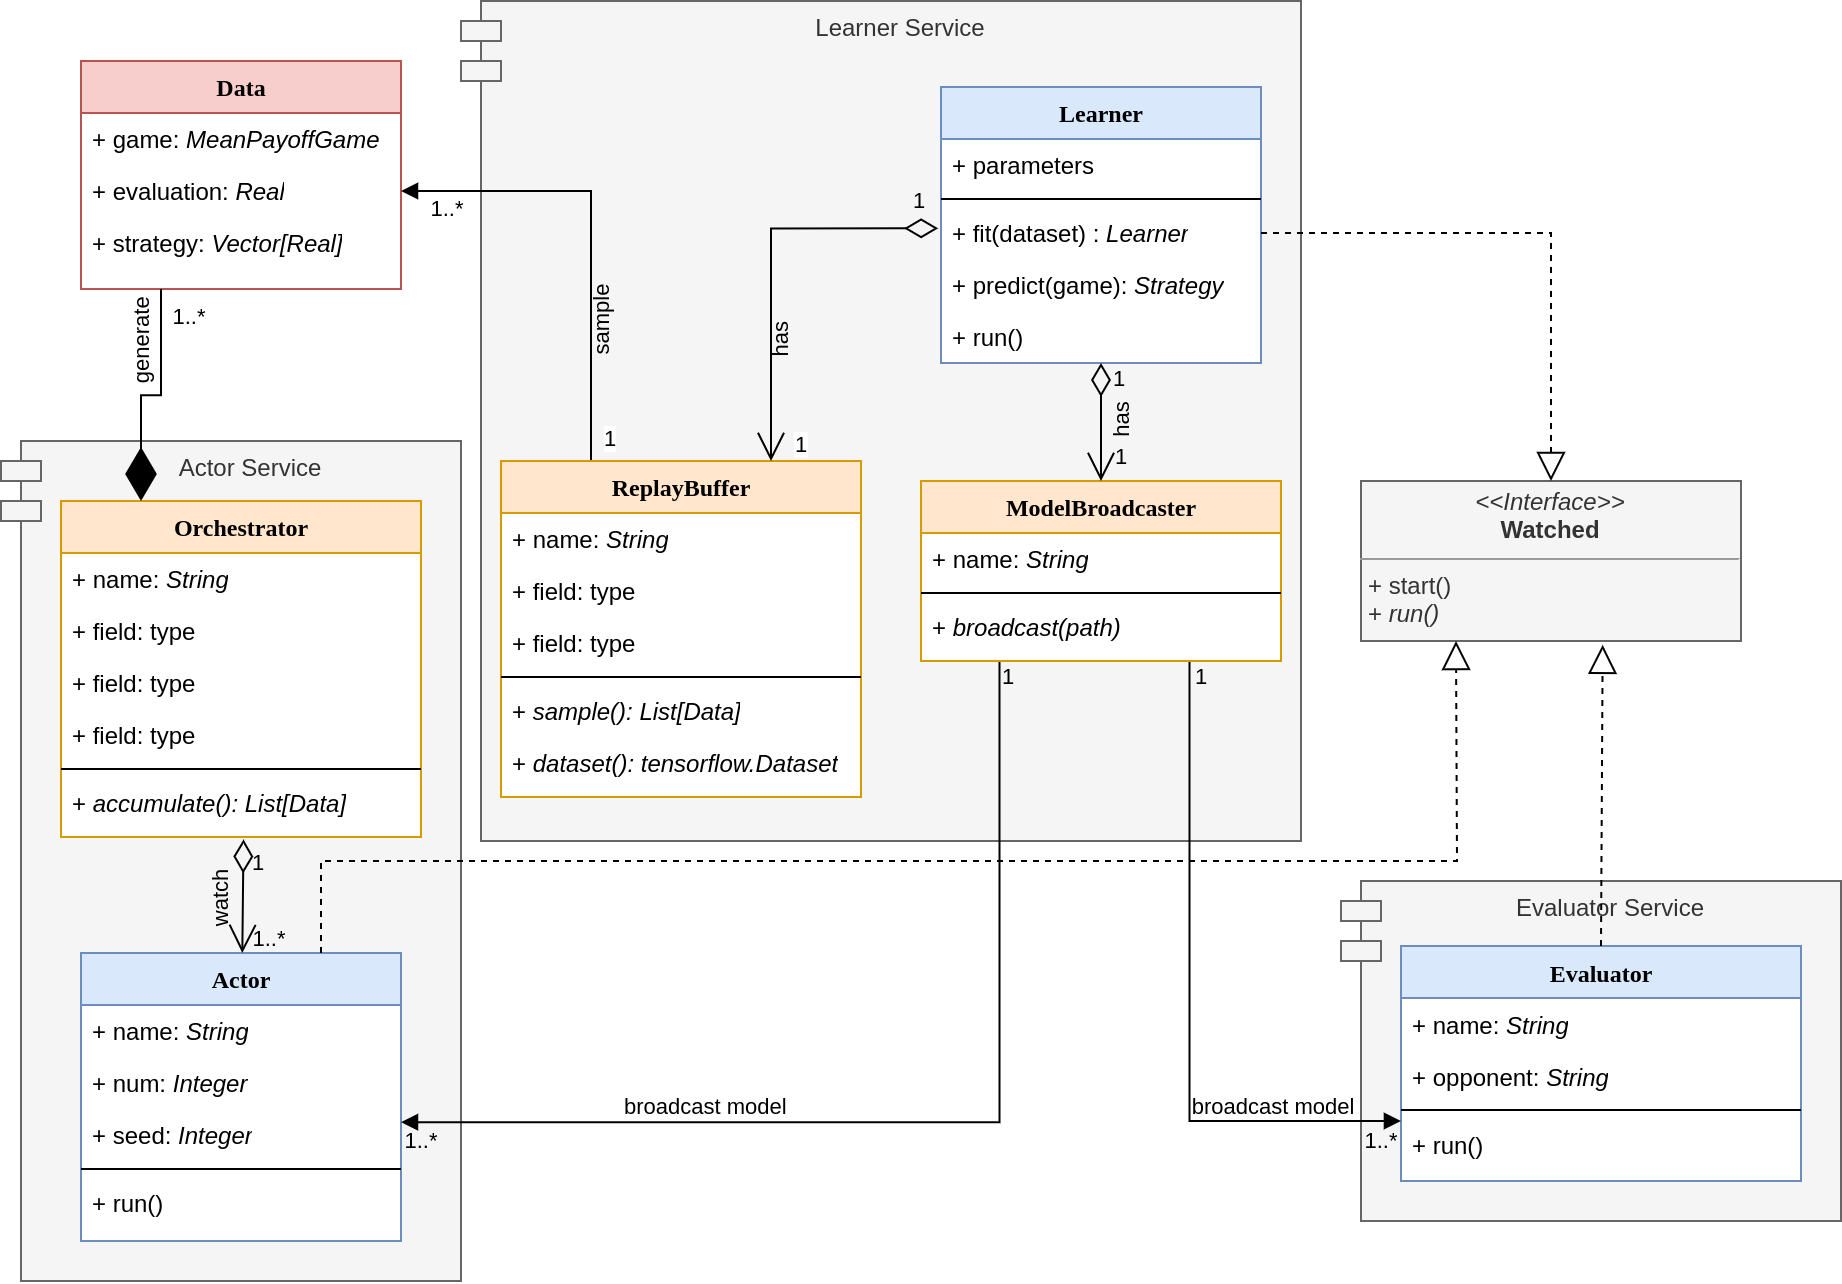
\includegraphics[width=0.85\textwidth]{Figures/ServiceRelations.png}
	\caption{Class }
\end{figure}
\FloatBarrier


\section{Pipeline}
\begin{figure}
	\centering
	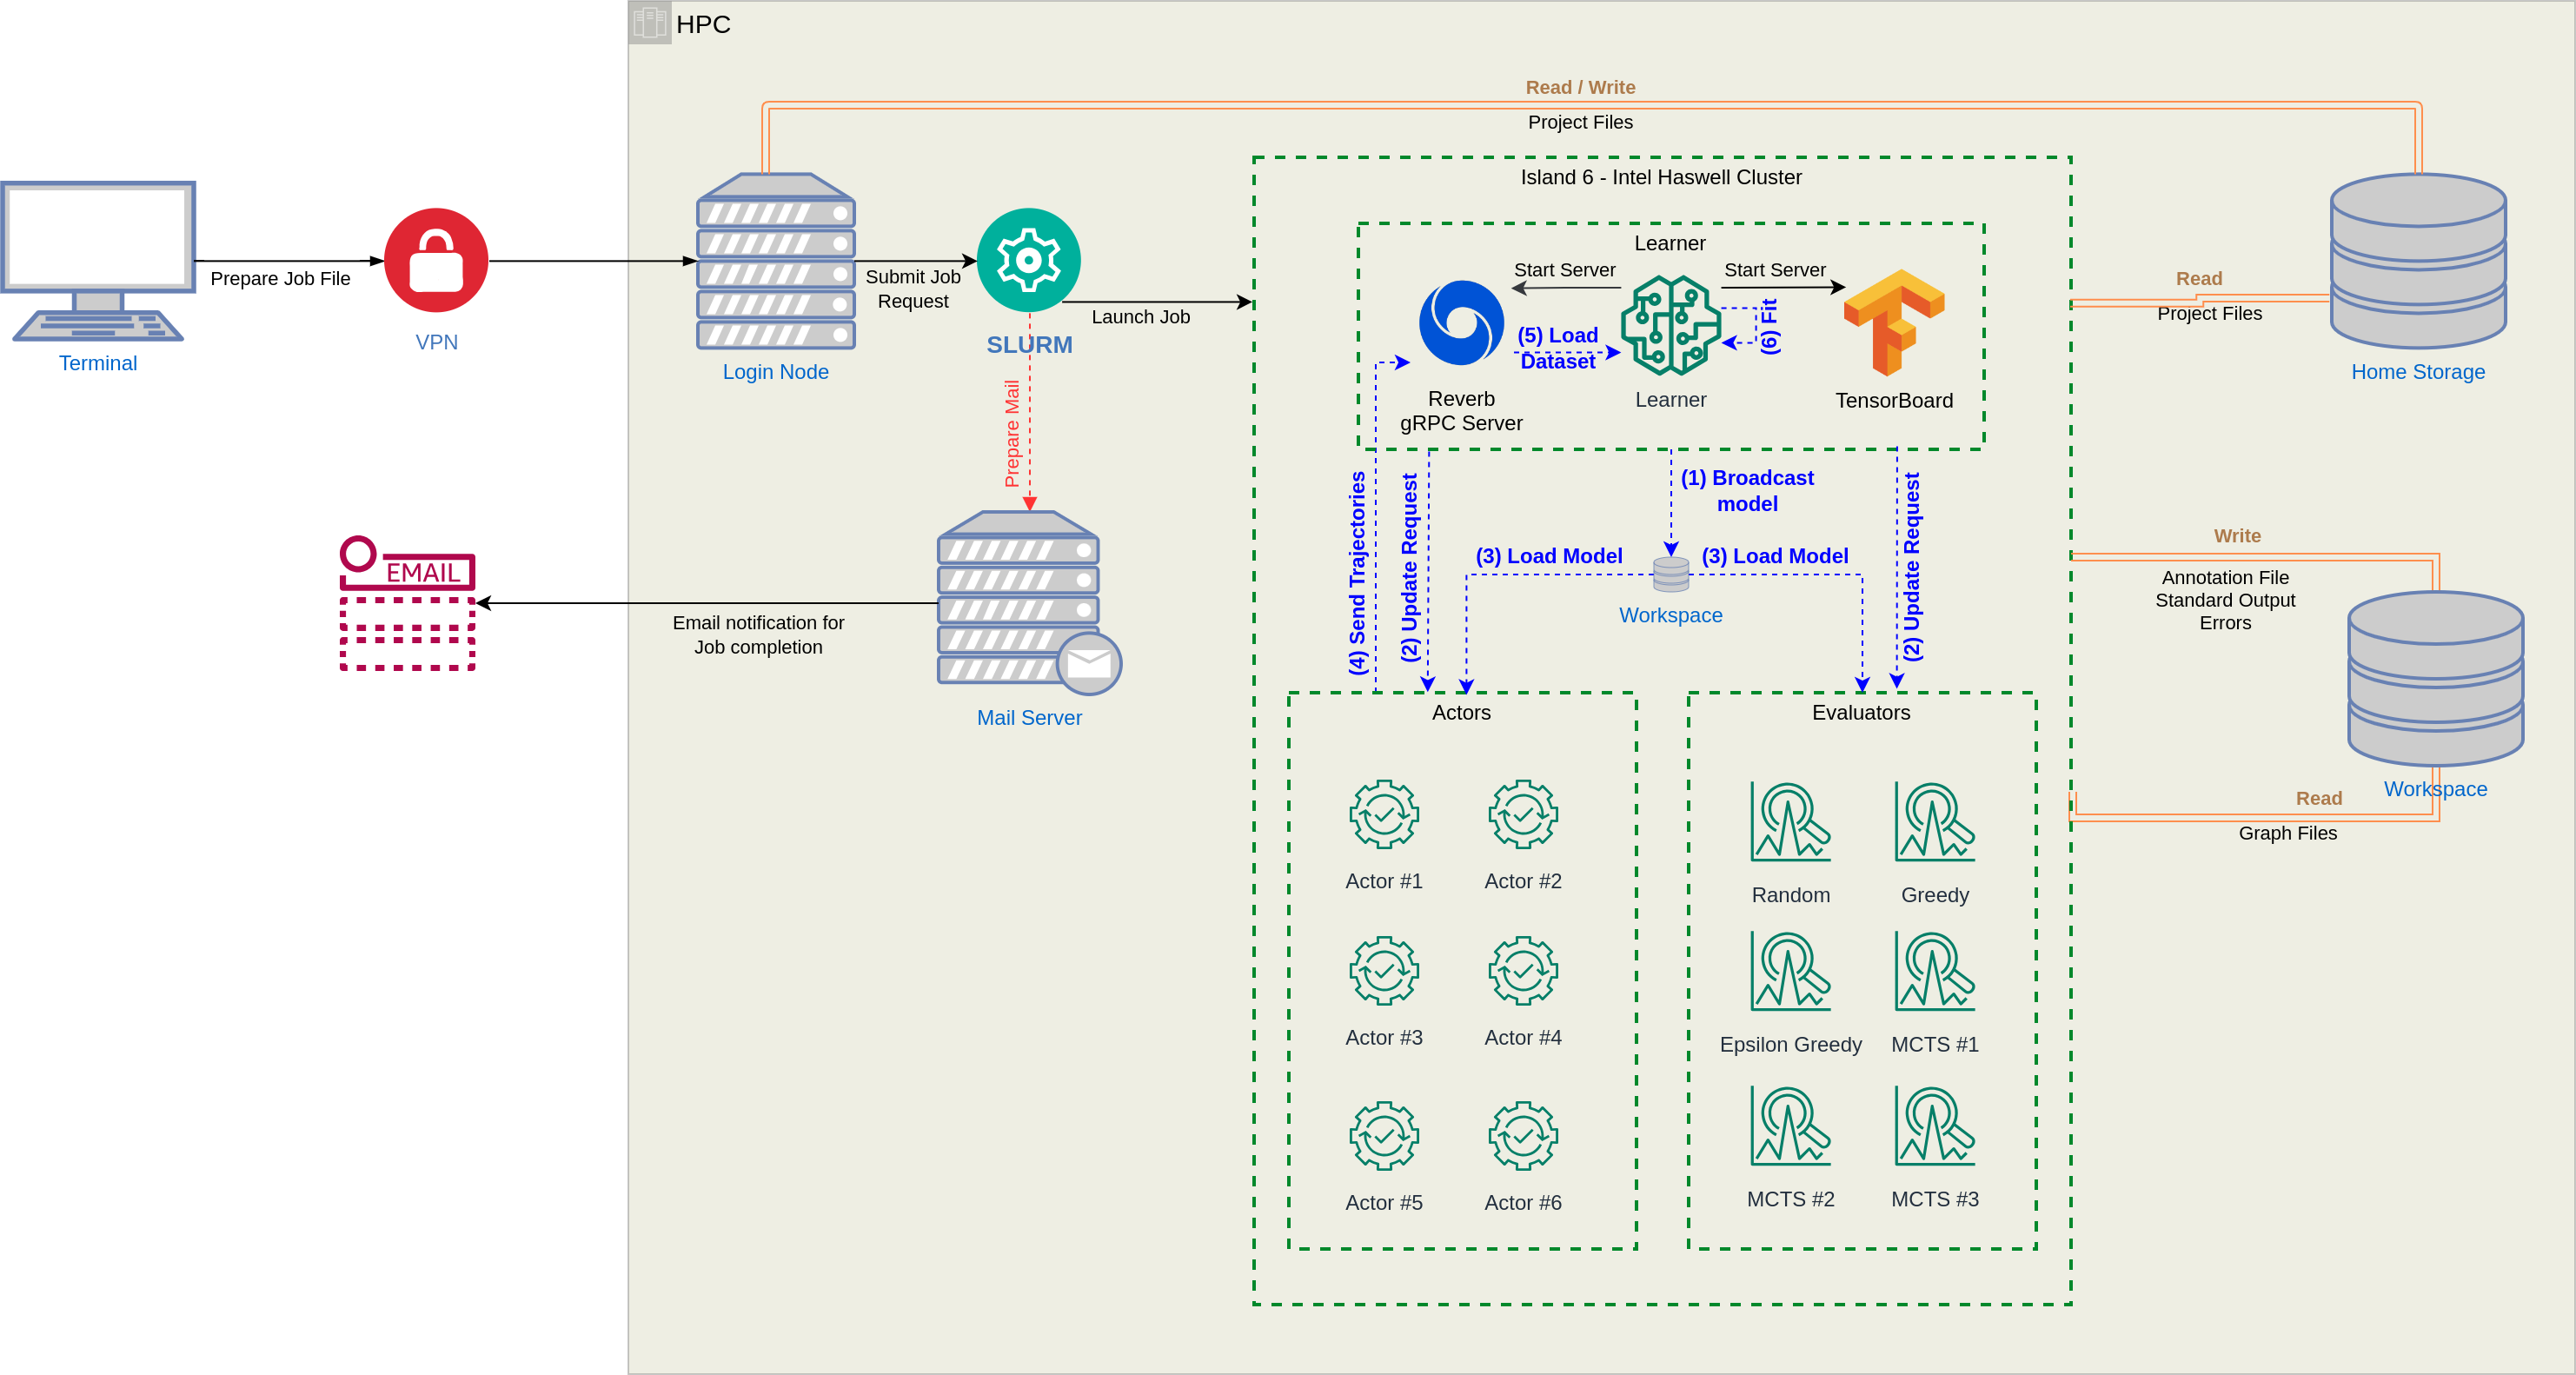
\includegraphics[width=0.95\textwidth]{Figures/AlphaZero.png}
	\caption{Pipeline Architecture}
\end{figure}
\section{Configuration}
